\documentclass{standalone}
\usepackage{tikz}
\usetikzlibrary{patterns, positioning}
\usepackage[sfdefault]{ClearSans} %% option 'sfdefault' activates Clear Sans as the default text font
\usepackage[T1]{fontenc}

\begin{document}
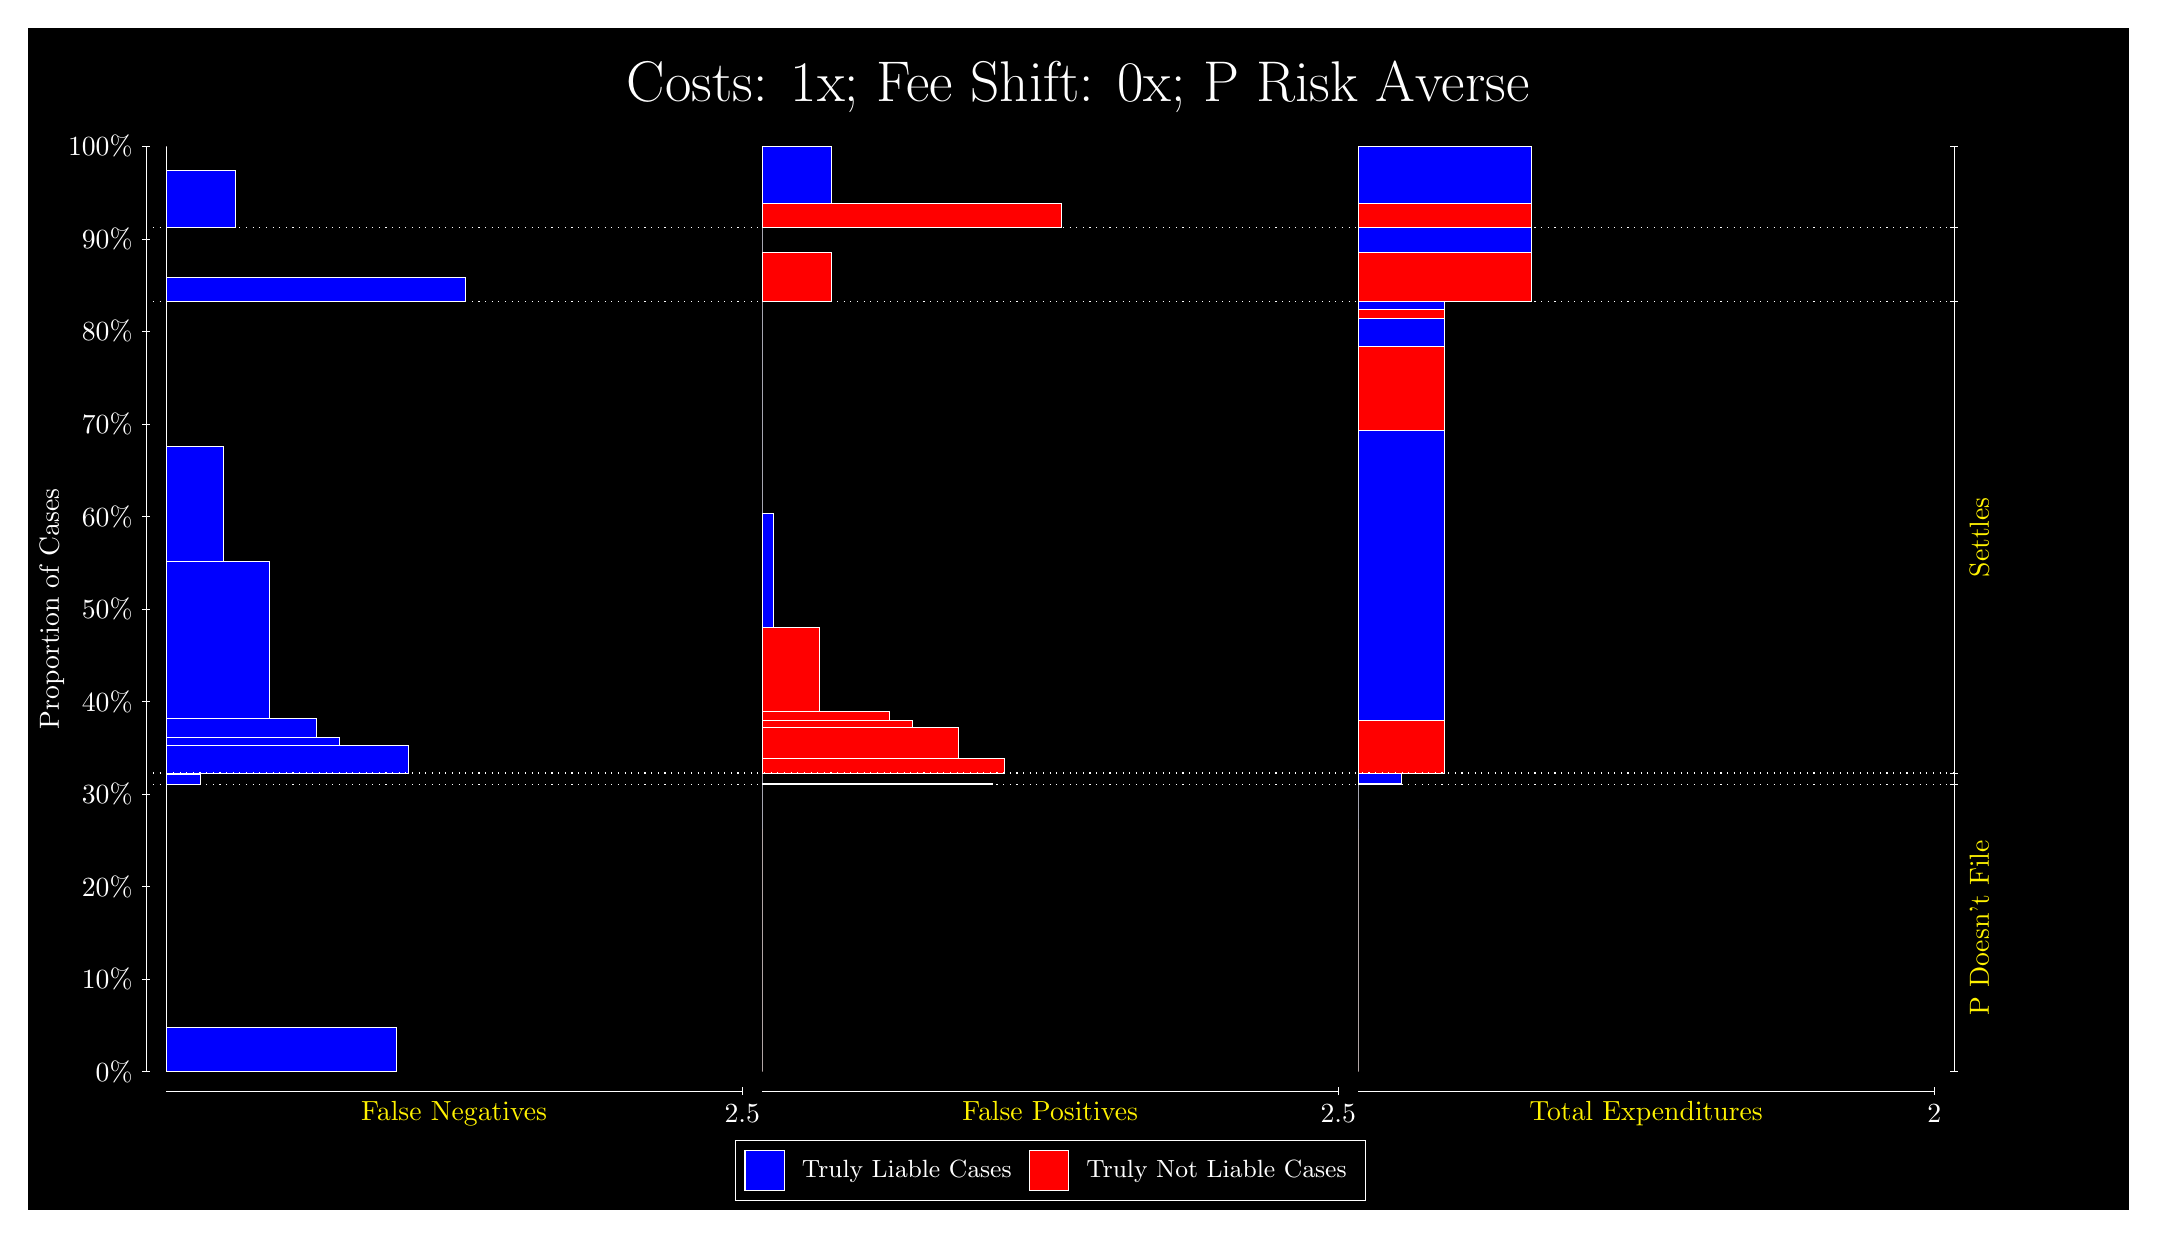
\begin{tikzpicture}
\draw[fill=black] (0,0) rectangle (26.667,15);
\draw[text=white] (0,13.5) rectangle (26.667,15) node[midway] {\huge Costs: 1x; Fee Shift: 0x; P Risk Averse};
\draw[white, very thin] (1.5,1.75) -- (1.5,13.5);
\node[rotate=90, text=white, anchor=center] at (0.3, 7.625) {Proportion of Cases};
\draw[white, very thin] (1.45,1.75) -- (1.55,1.75);
\node[text=white, anchor=east] at (1.45, 1.75) {0\%};
\draw[white, very thin] (1.45,2.925) -- (1.55,2.925);
\node[text=white, anchor=east] at (1.45, 2.925) {10\%};
\draw[white, very thin] (1.45,4.1) -- (1.55,4.1);
\node[text=white, anchor=east] at (1.45, 4.1) {20\%};
\draw[white, very thin] (1.45,5.275) -- (1.55,5.275);
\node[text=white, anchor=east] at (1.45, 5.275) {30\%};
\draw[white, very thin] (1.45,6.45) -- (1.55,6.45);
\node[text=white, anchor=east] at (1.45, 6.45) {40\%};
\draw[white, very thin] (1.45,7.625) -- (1.55,7.625);
\node[text=white, anchor=east] at (1.45, 7.625) {50\%};
\draw[white, very thin] (1.45,8.8) -- (1.55,8.8);
\node[text=white, anchor=east] at (1.45, 8.8) {60\%};
\draw[white, very thin] (1.45,9.975) -- (1.55,9.975);
\node[text=white, anchor=east] at (1.45, 9.975) {70\%};
\draw[white, very thin] (1.45,11.15) -- (1.55,11.15);
\node[text=white, anchor=east] at (1.45, 11.15) {80\%};
\draw[white, very thin] (1.45,12.325) -- (1.55,12.325);
\node[text=white, anchor=east] at (1.45, 12.325) {90\%};
\draw[white, very thin] (1.45,13.5) -- (1.55,13.5);
\node[text=white, anchor=east] at (1.45, 13.5) {100\%};

\draw[white, very thin] (24.457,1.75) -- (24.457,13.5);
\draw[white, very thin] (24.407,1.75) -- (24.507,1.75);
\node[anchor=west] at (24.407, 1.75) {};
\draw[white, very thin] (24.407,5.394) -- (24.507,5.394);
\node[anchor=west] at (24.407, 5.394) {};
\draw[white, very thin] (24.407,5.5416) -- (24.507,5.5416);
\node[anchor=west] at (24.407, 5.5416) {};
\draw[white, very thin] (24.407,11.53) -- (24.507,11.53);
\node[anchor=west] at (24.407, 11.53) {};
\draw[white, very thin] (24.407,12.468) -- (24.507,12.468);
\node[anchor=west] at (24.407, 12.468) {};
\draw[white, very thin] (24.407,13.5) -- (24.507,13.5);
\node[anchor=west] at (24.407, 13.5) {};

\draw[white, very thin, fill=blue] (1.75,1.75) rectangle (4.6775,2.3164);
\draw[white, very thin, fill=red] (1.75,2.3164) rectangle (1.75,5.394);
\draw[white, very thin, fill=blue] (1.75,5.394) rectangle (2.1891,5.5278);
\draw[white, very thin, fill=red] (1.75,5.5278) rectangle (1.75,5.5416);
\draw[white, very thin, fill=blue] (1.75,5.5416) rectangle (4.8239,5.8952);
\draw[white, very thin, fill=blue] (1.75,5.8952) rectangle (3.9457,5.9968);
\draw[white, very thin, fill=blue] (1.75,5.9968) rectangle (3.6529,6.2376);
\draw[white, very thin, fill=blue] (1.75,6.2376) rectangle (3.0674,8.2312);
\draw[white, very thin, fill=blue] (1.75,8.2312) rectangle (2.4819,9.6843);
\draw[white, very thin, fill=red] (1.75,9.6843) rectangle (1.75,11.53);
\draw[white, very thin, fill=blue] (1.75,11.53) rectangle (5.5558,11.839);
\draw[white, very thin, fill=red] (1.75,11.839) rectangle (1.75,12.468);
\draw[white, very thin, fill=blue] (1.75,12.468) rectangle (2.6283,13.19);
\draw[white, very thin, fill=red] (1.75,13.19) rectangle (1.75,13.5);
\draw[white, very thin, fill=red] (9.3189,1.75) rectangle (9.3189,4.8276);
\draw[white, very thin, fill=blue] (9.3189,4.8276) rectangle (9.3189,5.394);
\draw[white, very thin, fill=red] (9.3189,5.394) rectangle (12.246,5.4078);
\draw[white, very thin, fill=blue] (9.3189,5.4078) rectangle (9.3189,5.5416);
\draw[white, very thin, fill=red] (9.3189,5.5416) rectangle (12.393,5.7339);
\draw[white, very thin, fill=red] (9.3189,5.7339) rectangle (11.807,6.1203);
\draw[white, very thin, fill=red] (9.3189,6.1203) rectangle (11.222,6.2069);
\draw[white, very thin, fill=red] (9.3189,6.2069) rectangle (10.929,6.3242);
\draw[white, very thin, fill=red] (9.3189,6.3242) rectangle (10.051,7.3872);
\draw[white, very thin, fill=blue] (9.3189,7.3872) rectangle (9.4652,8.8403);
\draw[white, very thin, fill=blue] (9.3189,8.8403) rectangle (9.3189,11.53);
\draw[white, very thin, fill=red] (9.3189,11.53) rectangle (10.197,12.158);
\draw[white, very thin, fill=blue] (9.3189,12.158) rectangle (9.3189,12.468);
\draw[white, very thin, fill=red] (9.3189,12.468) rectangle (13.125,12.777);
\draw[white, very thin, fill=blue] (9.3189,12.777) rectangle (10.197,13.5);
\draw[white, very thin, fill=red] (16.888,1.75) rectangle (16.888,4.8276);
\draw[white, very thin, fill=blue] (16.888,4.8276) rectangle (16.888,5.394);
\draw[white, very thin, fill=red] (16.888,5.394) rectangle (17.437,5.4078);
\draw[white, very thin, fill=blue] (16.888,5.4078) rectangle (17.437,5.5416);
\draw[white, very thin, fill=red] (16.888,5.5416) rectangle (17.986,6.2069);
\draw[white, very thin, fill=blue] (16.888,6.2069) rectangle (17.986,9.8943);
\draw[white, very thin, fill=red] (16.888,9.8943) rectangle (17.986,10.957);
\draw[white, very thin, fill=blue] (16.888,10.957) rectangle (17.986,11.311);
\draw[white, very thin, fill=red] (16.888,11.311) rectangle (17.986,11.428);
\draw[white, very thin, fill=blue] (16.888,11.428) rectangle (17.986,11.53);
\draw[white, very thin, fill=red] (16.888,11.53) rectangle (19.083,12.158);
\draw[white, very thin, fill=blue] (16.888,12.158) rectangle (19.083,12.468);
\draw[white, very thin, fill=red] (16.888,12.468) rectangle (19.083,12.777);
\draw[white, very thin, fill=blue] (16.888,12.777) rectangle (19.083,13.5);
\draw[white, dotted] (1.5,5.394) -- (24.457,5.394);
\draw[white, dotted] (1.5,5.5416) -- (24.457,5.5416);
\draw[white, dotted] (1.5,11.53) -- (24.457,11.53);
\draw[white, dotted] (1.5,12.468) -- (24.457,12.468);
\draw[white, very thin] (1.75,1.5) -- (9.0689,1.5);
\node[text=yellow, anchor=north] at (5.4094, 1.5) {False Negatives};
\draw[white, very thin] (9.0689,1.45) -- (9.0689,1.55);
\node[text=white, anchor=north] at (9.0689, 1.45) {2.5};

\draw[white, very thin] (9.3189,1.5) -- (16.638,1.5);
\node[text=yellow, anchor=north] at (12.978, 1.5) {False Positives};
\draw[white, very thin] (16.638,1.45) -- (16.638,1.55);
\node[text=white, anchor=north] at (16.638, 1.45) {2.5};

\draw[white, very thin] (16.888,1.5) -- (24.207,1.5);
\node[text=yellow, anchor=north] at (20.547, 1.5) {Total Expenditures};
\draw[white, very thin] (24.207,1.45) -- (24.207,1.55);
\node[text=white, anchor=north] at (24.207, 1.45) {2};

\node[text=yellow, centered, rotate=90] at (24.777, 3.572) {P Doesn't File};

\node[text=yellow, centered, rotate=90] at (24.777, 8.5357) {Settles};



\draw (12.978300999999998,1.5) node[draw=none] (baseCoordinate) {};
\begin{scope}[align=center]
        \matrix[scale=0.5, draw=white, below=0.5cm of baseCoordinate, nodes={draw}, column sep=0.1cm]{
            \node[rectangle, draw, minimum width=0.5cm, minimum height=0.5cm, fill=blue] {}; &
            \node[draw=none, font=\small, text=white] (B) {Truly Liable Cases}; &
            \node[rectangle, draw, minimum width=0.5cm, minimum height=0.5cm, fill=red] {}; &
            \node[draw=none, font=\small, text=white] (B) {Truly Not Liable Cases}; \\
            };
\end{scope}

\end{tikzpicture}
\end{document}